% journal_body.tex — the body of the journal manuscript (Sections 1-8 with
% tables and figures), shared by paper.tex and measurement_manuscript.tex.
% journal_intro.tex — Section 1 of the journal manuscript (paper.tex).

\section{Introduction}
Evaluating measurement uncertainty by the propagation of distributions,
following Supplement~1 to the Guide to the Expression of Uncertainty in
Measurement (GUM~S1)~\cite{jcgm100,jcgm101}, requires the measurement model
$Y=f(\mathbf X)$ to be evaluated once per Monte Carlo trial, typically
$10^5$ to $10^6$ times~\cite{cox2006,harris2014}. For a growing class of
quantities $f$ is a numerical simulation. A computational fluid dynamics
(CFD) model of an accidental ammonia release in a factory~\cite{tan2017}
can take hours to days per run, so that a practical budget is a few tens of
runs, three or four orders of magnitude short of what the Monte Carlo
method needs. The same gap arises in scatterometry, where it has been
studied in detail~\cite{heidenreich2017}, and in many inverse and
model-based measurements.

The usual remedy is a \emph{surrogate} (emulator, metamodel) fitted to the
available runs and evaluated in place of $f$~\cite{ohagan2006,wang2022}.
Two questions then decide whether the resulting uncertainty statement can
be trusted: which surrogate reproduces the reported quantities best for a
given number of runs, and how the surrogate's own error is to be included
in the uncertainty budget, since it is not negligible at such budgets.
This paper answers both with a controlled comparison on ten models,
including a CFD dispersion case, and validates the answers against the
true models.

\subsection{Related work}
\emph{Gaussian process emulators.} Gaussian process (GP) regression, or
kriging, is the standard surrogate for deterministic computer
experiments~\cite{sacks1989,rw2006}. The Bayesian treatment of O'Hagan and
co-workers~\cite{ohagan2006,kennedy2001} reads the GP posterior as the
uncertainty about $f$ itself, which suggests using the posterior variance
as the surrogate contribution to an uncertainty budget. A common guideline
asks for about ten runs per input~\cite{loeppky2009}, and the effect of
modelling choices such as the correlation family, the mean function and
the treatment of the hyperparameters on GP accuracy has been assessed
systematically~\cite{chen2016}.

\emph{Polynomial chaos.} Polynomial chaos expansions (PCE) represent $Y$ in
polynomials orthonormal with respect to $g_{\mathbf X}$~\cite{xiu2002},
from which the moments and sensitivity indices follow
directly~\cite{sudret2008}. With few runs, sparse expansions selected by
least-angle regression~\cite{efron2004} and a corrected leave-one-out
error are the method of choice~\cite{blatman2011}.

\emph{Ensembles and committees.} Combining several surrogates with weights
derived from their cross-validation errors protects against choosing a poor
surrogate~\cite{goel2007,viana2009}; the spread of the members has also
been used as an interval for the output, in the spirit of probability
boxes~\cite{ferson1996}.

\emph{Adaptive designs.} Instead of fixing all runs in advance, runs can be
added where the surrogate is most uncertain, by its posterior
variance~\cite{gramacy2009}, by the disagreement of a committee, or by
measures such as the spectral uncertainty of Lin et al.~\cite{lin2024}. For
the probability of exceeding a threshold, the AK-MCS method of Echard et
al.~\cite{echard2011} places runs where the sign of $f-T$ is most
uncertain.

\emph{Validity of the surrogate contribution.} Whether any of these
uncertainty descriptions has the coverage it claims is rarely checked
against the true model. Conformal prediction~\cite{angelopoulos2023}, and
in particular the jackknife+~\cite{barber2021}, gives prediction intervals
with a coverage guarantee that holds for any fitted model, using only
leave-one-out fits. To our knowledge it has not been compared with GP
posterior intervals as the surrogate contribution in a GUM~S1 evaluation.

\emph{Benchmarks.} Comparisons of surrogates are sensitive to the test
functions and to the number of repetitions. We use standard functions from
the literature~\cite{vlse,wicaksono2023}, GUM-type input distributions, a
physical dispersion formula and a CFD case, with 30 paired repetitions and
statistics adjusted for multiple comparisons.

\subsection{Earlier analysis and contributions}
An earlier analysis by the first author combined a heterogeneous committee,
the spectral acquisition criterion and dynamic model management, and
reported that a passively sampled GP fails catastrophically on large input
domains, a failure the committee avoided. The present study re-examines
these claims with correctly specified baselines and extends them to the
general question above. Its contributions are:
\begin{enumerate}\setlength\itemsep{1pt}
\item a paired comparison, on ten models with uniform and GUM-type inputs
and a CFD dispersion case, of GP specifications, sparse PCE, committees and
adaptive and targeted designs at budgets of 10 to 80 runs, scored on the
quantities a GUM~S1 evaluation reports;
\item the finding that the GP failure of the earlier analysis is a
kernel-specification artefact, and that specification (amplitude,
anisotropy, trend) and variable transformation matter more than the choice
between single surrogates, committees and adaptive designs;
\item a validation, against the true models, of three ways to include the
surrogate error in GUM~S1: the GP posterior, a cross-validation (CV)
normal error and resampled leave-one-out residuals, with jackknife+
intervals as a distribution-free reference;
\item a procedure for surrogate-based GUM~S1 evaluations
(Fig.~\ref{fig:flowchart}), and code, per-seed records and an audit script
that recompute every number reported~\cite{repo}.
\end{enumerate}

% journal_methods.tex — Sections 2-4 of the journal manuscript (paper.tex),
% kept in a separate file while the results sections are written.

\section{Surrogate-based propagation and the surrogate contribution}
\label{sec:framework}
\subsection{Propagation of distributions through a surrogate}
Let $Y=f(\mathbf X)$ be the measurement model, $g_{\mathbf X}$ the joint
probability density of the inputs (here with independent components) and
$\{(\mathbf x_i,y_i)\}_{i=1}^N$, $y_i=f(\mathbf x_i)$, the $N$ available
model runs. A surrogate $\hat f$ is fitted to the runs and the Monte Carlo
method of GUM~S1~\cite{jcgm101} is applied to $\hat f$: $M$ draws
$\mathbf x^{(r)}\sim g_{\mathbf X}$ give $\hat y^{(r)}=\hat f(\mathbf x^{(r)})$,
from which the estimate $y$ (the mean), the standard uncertainty $u(y)$ (the
standard deviation), the probabilistically symmetric 95\% coverage interval
$[y_{0.025},y_{0.975}]$, the 95th percentile $y_{0.95}$ and the probability
$P(Y>T)$ of exceeding a threshold $T$ are computed. We call these the
\emph{reported quantities}.

Surrogates are fitted on a \emph{latent} scale $z=\varphi(y)$, with
$\varphi=\log$ for the log-variable variants and the identity otherwise, and
predictions are mapped back by $\varphi^{-1}$. For a Gaussian latent
predictive distribution, $\exp$ of the latent mean is the predictive median
of $Y$; no bias correction is applied.

\subsection{The surrogate error as an uncertainty contribution}
\label{sec:contrib}
The surrogate error $e(\mathbf x)=\varphi(f(\mathbf x))-\varphi(\hat f(\mathbf x))$
is unknown. Following Kennedy and O'Hagan~\cite{kennedy2001}, who treat model
inadequacy as an uncertainty source, we propagate
\begin{equation}
Y=\varphi^{-1}\!\left(\varphi(\hat f(\mathbf X))+E\right),
\label{eq:contrib}
\end{equation}
with $E$ a random variable describing the surrogate error, drawn
independently for every Monte Carlo trial. Three models for $E$ are
compared, all available from the $N$ runs alone:
\begin{itemize}\setlength\itemsep{1pt}
\item \emph{GP}: $E\mid\mathbf x\sim\mathrm N(0,s^2(\mathbf x))$, with
$s(\mathbf x)$ the predictive SD of a Gaussian process surrogate;
\item \emph{CV-normal}: $E\sim\mathrm N(0,s_{\mathrm{LOO}}^2)$, with
$s_{\mathrm{LOO}}^2=N^{-1}\sum_i r_i^2$ and
$r_i=\varphi(y_i)-\varphi(\hat f_{-i}(\mathbf x_i))$ the leave-one-out (LOO)
residuals; $\hat f_{-i}$ is the surrogate re-fitted, hyperparameters
included, without run $i$;
\item \emph{resampling}: $E$ drawn with equal probabilities from
$\{r_1,\dots,r_N\}$.
\end{itemize}
The same ingredients give pointwise 95\% prediction intervals for
$f(\mathbf x)$: the GP interval $\hat z\pm1.96\,s(\mathbf x)$, the CV-normal
interval $\hat z\pm1.96\,s_{\mathrm{LOO}}$, and the jackknife+
interval~\cite{barber2021}
\begin{equation}
\left[\,q^-_{\alpha}\{\hat z_{-i}(\mathbf x)-|r_i|\},\;
q^+_{\alpha}\{\hat z_{-i}(\mathbf x)+|r_i|\}\,\right],
\end{equation}
where $q^-_\alpha$ is the $\lfloor\alpha(N+1)\rfloor$-th smallest and
$q^+_\alpha$ the $\lceil(1-\alpha)(N+1)\rceil$-th smallest of the $N$ values,
$\alpha=0.05$. For exchangeable runs the jackknife+ interval covers $f$ with
probability at least $1-2\alpha$ whatever the surrogate~\cite{barber2021};
it is a member of the conformal family~\cite{angelopoulos2023}.

\emph{Why resampling the LOO residuals can be expected to work.} For an
input $\mathbf X\sim g_{\mathbf X}$ drawn independently of the runs,
$\varphi(f(\mathbf X))=\varphi(\hat f(\mathbf X))+e(\mathbf X)$ exactly, so
equation~\eqref{eq:contrib} gives the true distribution of the output if $E$
behaves as $e(\mathbf X)$. If the run inputs and $\mathbf X$ are
exchangeable, as for independent draws from $g_{\mathbf X}$, each $r_i$ is
distributed as the error of a surrogate fitted to $N-1$ runs at a new input,
so the empirical distribution of the $r_i$ estimates the distribution of
$e(\mathbf X)$, on the conservative side because $N-1$ rather than $N$ runs
are used~\cite{arlot2010}. Three approximations remain. Resampling draws $E$
independently of $\mathbf X$: it reproduces the variance of the error but
drops its covariance with $\varphi(\hat f(\mathbf X))$, which is zero in
expectation when $\hat f$ is the posterior mean of a correctly specified
model but not in general. A Latin hypercube design is close to, not exactly,
exchangeable with independent draws. And a feature of $f$ that no run
reaches leaves no trace in any $r_i$ (Section~\ref{sec:res-robust}). At a
fixed input $\mathbf x$, the same construction with $\hat f_{-i}(\mathbf x)$
in place of $\hat f(\mathbf x)$ is the predictive distribution behind the
jackknife+ interval, one of the conformal predictive distributions, which
are valid in finite samples under exchangeability~\cite{barber2021,vovk2019}.
For the distribution of $Y$, which mixes over the inputs, no such guarantee
is available, and the coverage study of Section~\ref{sec:res-coverage} is
its empirical check.

For a reported quantity $\theta$ itself (the mean, SD, $y_{0.95}$ or
$P(Y>T)$ of the output over a fixed set of input draws), two 95\% intervals
are compared: the 2.5th and 97.5th percentiles of $\theta$ over joint sample
paths of the GP posterior, and the jackknife interval
$\hat\theta\pm1.96\,\mathrm{SE}_{\mathrm J}$ with
$\mathrm{SE}_{\mathrm J}^2=\frac{N-1}{N}\sum_i(\hat\theta_{-i}-\bar\theta)^2$,
where $\hat\theta_{-i}$ is computed from $\hat f_{-i}$.

\emph{Hyperparameter uncertainty.} The GP intervals above plug in the
maximum-likelihood (ML) hyperparameters, which may make them too narrow
with few runs. Three variants test whether the GP's shortfall is a plug-in
effect: (i) a Student-t process, with the overall variance scale and a
constant mean integrated out under the reference prior
$p(\beta,\sigma^2)\propto\sigma^{-2}$ and the correlation hyperparameters at
their ML values (the standard Bayesian emulator~\cite{ohagan2006}, $N-1$
degrees of freedom); (ii) a fully Bayesian GP, all hyperparameters
integrated out by Markov chain Monte Carlo (affine-invariant ensemble
sampler~\cite{foremanmackey2013}, uniform prior on each log-hyperparameter
within the ML search range, 800 steps of which 300 burn-in, 200 posterior
draws; $N=20$ only, for cost); and (iii) the GP SD recalibrated by the LOO
standardised residuals $z_i=r_i/s_{-i}(\mathbf x_i)$: pointwise
$\hat z\pm q\,s(\mathbf x)$ with $q$ the $\lceil0.95(N+1)\rceil$-th
smallest $|z_i|$, $E=s(\mathbf x)\,z_J$ in equation~\eqref{eq:contrib}, and
sample paths with the covariance scaled by the mean of $z_i^2$. The last is
a hybrid that keeps the GP's localisation of the error and takes its scale
from the runs. Each variant is assessed in the same three ways.

\section{Test models}
\label{sec:models}
Table~\ref{tab:models} lists the twelve models. Eight have independent uniform
inputs, three have the non-uniform input distributions of a GUM-type
evaluation, and one is a CFD simulation. The physics model is the benchmark
of the earlier analysis; its quadratic term carries practically all the
output variance on $[-200,200]^3$ and lies in the class of a degree-2
polynomial. The plume model is the ground-level concentration of a
continuous ammonia release from a Gaussian plume with ground reflection,
\begin{equation}
C=\frac{10^3\,Q}{2\uppi\,u\,\sigma_y\sigma_z}
\exp\!\left(-\frac{y^2}{2\sigma_y^2}\right)
2\exp\!\left(-\frac{H^2}{2\sigma_z^2}\right)\ \mathrm{mg\,m^{-3}},
\end{equation}
with Briggs rural coefficients for neutral stability,
$\sigma_y=0.08x(1+10^{-4}x)^{-1/2}$ and $\sigma_z=0.06x(1+1.5\times10^{-3}x)^{-1/2}$.
The borehole~\cite{harper1983,morris1993,vlse},
Ishigami~\cite{vlse}, OTL circuit and piston~\cite{benari2007} and wing
weight~\cite{forrester2008} functions are standard test functions for
computer experiments. To test whether the results hold when the inputs
outnumber what 20 runs can resolve, the OTL circuit is also run with 14
additional inputs that do not affect the output (uniform on $[100,200]$,
as in the screening study of Moon~\cite{moon2010}), so that $d=20$ and
$N=20$ is one run per input. The flood
model~\cite{iooss2015} gives the maximal annual underflow of a river with
truncated Gumbel, truncated normal, triangular and uniform inputs. The
borehole model is also run with the input model of Harper and
Gupta~\cite{harper1983} (normal borehole radius, lognormal radius of
influence) and the plume model with GUM-type inputs: lognormal emission rate
(median 500\,g\,s$^{-1}$, geometric SD 2), a Weibull wind speed (shape 2,
scale 4\,m\,s$^{-1}$, truncated to $[0.5,15]$\,m\,s$^{-1}$) and a normal
crosswind offset (SD 15\,m). All formulas and input models were checked
against the independent implementation in UQTestFuns~\cite{wicaksono2023}
(relative differences below $10^{-10}$ for outputs and $10^{-6}$ for
marginal quantiles).

A further analytical model, reported separately, tests the limits of the
procedure: a smooth
function of four uniform inputs on $[0,1]^4$ plus a narrow Gaussian bump,
$f=x_1+x_2^2+0.5\sin(2\uppi x_3)+0.5x_4+3.6\exp(-\lVert\mathbf x-0.7\rVert^2/(2\cdot0.13^2))$.
The bump carries about 10\% of the output variance in a region (bump above
10\% of its height) of 3\% of the input volume, which a Latin hypercube of
20 runs misses with probability 0.53 and one of 40 runs with probability
0.26 (Section~\ref{sec:res-robust}).
Two variants test assumptions of the main study. In the first, the inputs
are dependent: the borehole model with GUM-type inputs, with a Gaussian
copula of correlation 0.5 between the two transmissivities and between the
two heads. Designs are drawn in the space of independent uniform variables
and mapped to the inputs by the inverse Rosenblatt transformation of the
copula, so the surrogates and the propagation are otherwise unchanged. In
the second, the output is a vector: the plume model at three receptors on
the plume axis, at $x$, $x+200$\,m and $x+400$\,m, gives three strongly
correlated output quantities, propagated as in GUM~S2~\cite{jcgm102}. Each
component has its own log-scale GP, and the surrogate error is added on the
log scale in one of three ways: as the LOO residual vector of one run, drawn
with equal probabilities (\emph{joint} resampling, which keeps the
correlation between the components), as residuals drawn independently for
each component, or as independent normal errors with the LOO RMS error of
each component. The coverage region is the hyperellipsoidal region of
GUM~S2, from the mean and covariance matrix of the propagated sample with
the coverage factor set so that 95\% of the sample lies inside, computed on
the original and on the log scale. Its achieved coverage is evaluated under
$2\times10^5$ draws of the true model, and its volume is compared with that
of the same region computed from the true model.

Exceedance is assessed at a fixed threshold where the model has one (the
IDLH level for ammonia, 210\,mg\,m$^{-3}$, about 300\,ppm, for the plume
and CFD models), and otherwise at the reference 95th percentile, for which
$P(Y>T)=0.05$ by construction. Flooding has a probability below $10^{-5}$
for the flood input model, so its threshold is the reference 5th percentile
of the underflow, $P(Y<T)=0.05$.

\begin{table*}[tb]
\centering
\caption{Test models. $d$: number of inputs; U: independent uniform inputs.
The models below the line test the limits and assumptions of the procedure
and are reported separately.}
\label{tab:models}
\small
\begin{tabular}{llp{53mm}p{54mm}}
\toprule
Model & $d$ & Inputs & Character\\
\midrule
Physics & 3 & U$[-200,200]^3$, noise SD 0.1 & quadratic bowl plus small oscillatory terms\\
Plume & 5 & U: $Q$, $u$, $H$, $x$, $y$ & multiplicative, positive, heavy right tail\\
Borehole & 8 & U, ranges of~\cite{vlse} & smooth, multiplicative, positive\\
Ishigami & 3 & U$[-\uppi,\uppi]^3$ & strongly non-linear, interactions\\
OTL circuit & 6 & U~\cite{benari2007} & smooth, nearly additive, positive\\
Piston & 7 & U~\cite{benari2007} & non-linear, positive\\
Wing weight & 10 & U~\cite{forrester2008} & smooth, multiplicative, positive\\
OTL circuit, 20 inputs & 20 & U, 14 inactive~\cite{moon2010} & as OTL circuit; sparse\\
Borehole (GUM) & 8 & normal, lognormal, uniform~\cite{harper1983} & as borehole; input tails\\
Plume (GUM) & 5 & lognormal, truncated Weibull, uniform, normal & as plume; heavier input and output tails\\
Flood & 8 & truncated Gumbel and normal, triangular, uniform~\cite{iooss2015} & smooth, lower-tail threshold\\
CFD dispersion & 6 & U: $U_{\mathrm{ref}}$, $z_0$, $H_{\mathrm b}$, $Sc_t$, $x_r$, $Q$ & RANS solution: wake recirculation, numerical error\\
\midrule
Bump (failure mode) & 4 & U$[0,1]^4$ & smooth part plus a narrow bump that the runs can miss\\
Borehole, dependent & 8 & as Borehole (GUM), Gaussian copula & dependent inputs\\
Plume, 3 receptors & 5 & as Plume & vector output (GUM~S2)\\
\bottomrule
\end{tabular}
\end{table*}

\subsection{CFD dispersion case}
\label{sec:cfd}
The CFD case replaces the plume formula by a Reynolds-averaged
Navier--Stokes (RANS) simulation of a continuous ground-level release
upwind of a building, solved with OpenFOAM v1912~\cite{weller1998}. The
domain is two-dimensional (a vertical plane along the wind; the building
and the release are infinitely wide), from 80\,m upstream to 250\,m
downstream of the windward face and 150\,m high. The building is 10\,m deep
and $H_{\mathrm b}$ high; the release is a unit line source 20\,m upstream
of the building, 0.5\,m above the ground. The inflow is the neutral
atmospheric surface layer of Richards and Hoxey~\cite{richards1993},
$U(z)=(u_*/\kappa)\ln((z+z_0)/z_0)$, $k=u_*^2/\sqrt{C_\mu}$,
$\varepsilon=u_*^3/(\kappa(z+z_0))$, scaled to the wind speed
$U_{\mathrm{ref}}$ at 10\,m, with the standard $k$--$\varepsilon$ model
($\sigma_\varepsilon=1.11$ for consistency with the inflow), a rough-wall
function on the ground~\cite{blocken2007}, smooth building walls and a slip
top boundary. The concentration $s$ of the passive scalar solves
$\nabla\cdot(\mathbf U s)-\nabla\cdot((\nu/Sc+\nu_t/Sc_t)\nabla s)=S$, with
$Sc=0.7$ and the turbulent Schmidt number $Sc_t$ as an input, since its
appropriate value is uncertain and varies between flows~\cite{tominaga2007}.
Flow and scalar are solved together by the SIMPLE algorithm on 7776
hexahedral cells, refined towards the building, until all scaled residuals
fall below $10^{-5}$ (pressure) and $10^{-6}$ (other fields), or 4000
iterations, typically in
1000--1500 iterations (about 20\,s on one core). The output is the
concentration at 1.5\,m height a distance $x_r$ downstream of the leeward
face, $C=10^3\,Q\,s(x_r)$\,mg\,m$^{-3}$ for a release rate $Q$ per metre of
crosswind width; since the scalar is passive, $x_r$ and $Q$ need no
separate run. The six inputs are uniform: $U_{\mathrm{ref}}\in[1,6]$\,m\,s$^{-1}$,
$z_0\in[0.01,0.3]$\,m, $H_{\mathrm b}\in[6,15]$\,m, $Sc_t\in[0.5,1.3]$,
$x_r\in[5,120]$\,m and $Q\in[1,20]$\,g\,s$^{-1}$\,m$^{-1}$.

The case contains what the plume formula lacks: flow separation at the
building edges, a recirculating wake whose length and strength change with
$H_{\mathrm b}$ and $z_0$, receptors inside and beyond the wake, and a
discretisation and iteration error that varies with the inputs. It is a
benchmark, not a validated prediction of a particular site: the model is
\emph{defined} as this discretised RANS solution, which is what a surrogate
of an expensive simulation has to reproduce. A reference Monte Carlo of
$2\times10^5$ CFD runs is not affordable. The reference distribution is
built instead from 800 runs at independent uniform draws of the four flow
inputs, each combined with 50 independent draws of $(x_r,Q)$: 40\,000
reference points, of which 4000 (five per run) form the test set and 1600
(two per run) the input set for derived quantities. The grid sensitivity of
the case is reported in Section~\ref{sec:res-cfd}.

\section{Surrogates, designs and protocol}
\label{sec:protocol}
\subsection{Surrogates}
\paragraph{Gaussian processes.} All GPs are fitted on standardised inputs
and outputs by maximising the log marginal likelihood (L-BFGS-B, five
random restarts) with scikit-learn. The specifications, in order of
increasing completeness, are: (i) the \emph{original} kernel of the earlier
analysis, a squared exponential with one length scale and an amplitude
\emph{fixed} at 1 on the standardised output; (ii) with the amplitude
estimated; (iii) with one length scale per input (automatic relevance
determination, ARD) but the amplitude fixed; (iv) with both; (v) a
Mat\'ern-5/2 ARD kernel with amplitude and a nugget; (vi) (v) plus an
amplitude-scaled quadratic polynomial kernel, i.e.\ a GP with a quadratic
trend whose coefficients are integrated out. Length scales are bounded to
$[10^{-2},10^3]$, the amplitude to $[10^{-3},10^3]$ and the nugget variance
to $[10^{-8},10^{-1}]$. Variants (v) and (vi) are also fitted on the log
scale for positive outputs, with logarithmic transformation of inputs whose
support is positive.

\paragraph{Sparse polynomial chaos.} A sparse PCE~\cite{blatman2011} with an
orthonormal Legendre basis on inputs mapped to $[-1,1]$ (affinely for
uniform inputs, through their distribution functions otherwise), candidate
sets of total degree $p=1,\dots,5$ with hyperbolic truncation ($q=1$ for
$p\le2$, $q=0.75$ above), least-angle regression~\cite{efron2004} to order
the basis terms, ordinary least squares on every active set along the path,
and selection of the active set and degree by the corrected LOO
error~\cite{blatman2011}. It is fitted on the raw and on the log scale.

\paragraph{Committees.} Nine members: two GPs (squared exponential and
Mat\'ern-3/2, both ARD with amplitude), PCEs~\cite{xiu2002,sudret2008} of degrees 2
and 3 (Bayesian ridge regression), random forests of 50 and 100 trees, a
support vector regressor and two neural networks. Members are combined
uniformly or with weights
$w_k\propto[\mathrm{MSE}_{\mathrm{CV},k}(1+\pi_k)]^{-1}$, with
$\mathrm{MSE}_{\mathrm{CV},k}$ the three-fold cross-validation error of
member $k$ and $\pi_k\ge0$ a penalty for predictions below a known
physical bound~\cite{goel2007,viana2009}.

\paragraph{Stacking.} As an alternative to choosing one candidate surrogate
(Section~\ref{sec:res-select}), the candidates are combined by
stacking~\cite{breiman1996}: non-negative weights that minimise the squared
error of the weighted sum of their LOO predictions (non-negative least
squares) are applied to the candidates fitted to all runs.

\subsection{Designs}
Passive designs are $N$-point Latin hypercubes drawn on $[0,1]^d$ and mapped
to the inputs by the inverse distribution functions. Adaptive designs start
from $N_0$ Latin hypercube runs ($N_0=5$ for $N\le20$, $N/4$ above) and add
one run at a time, refitting after every run: \emph{GP-SD} adds the
candidate with the largest posterior SD~\cite{gramacy2009}; the adaptive
committees add the candidate where the active members disagree most, by the
variance of their predictions or by the spectral measure
UEigV~\cite{lin2024} of the earlier analysis; and \emph{AK-MCS} adds the
candidate minimising $|\hat z(\mathbf x)-\varphi(T)|/s(\mathbf x)$, the
learning function of Echard et al.~\cite{echard2011}, which concentrates
runs near the threshold $T$ of the exceedance probability. \emph{IMSE}
adds the candidate that most reduces the integrated posterior variance of
the GP~\cite{sacks1989}, averaged over 1000 draws from the input
distribution, a criterion aimed at the whole distribution of the output
rather than at the largest local uncertainty. Candidates are random draws
from the input distribution (300 for GP-SD and IMSE, 2000 for AK-MCS).
To test whether the results depend on the type of passive design, the
Latin hypercube is replaced, in a separate comparison at $N=20$, by the
maximin Latin hypercube~\cite{morris1995} (the one with the largest
smallest distance between two runs among 200 random ones) and by the first
$N$ points of a randomly scrambled Sobol' sequence~\cite{sobol1967}.

\subsection{Protocol and statistics}
Every strategy is run with the 30 seeds 1000--1029 and budgets
$N=10,20,40,80$ (the full set of strategies at $N=20$). Seeds are shared and
the Latin hypercube is seeded from the global random state, so that for a
given seed all passive strategies use the identical design and all adaptive
strategies the identical start. Accuracy over the input domain is the root
mean square error on 5000 test points divided by the reference output SD
(normalised RMSE, nRMSE; 1 corresponds to a constant predictor). The
surrogates propagate $3\times10^4$ input draws; the reference uses
$2\times10^5$ draws of the model (Section~\ref{sec:cfd} for the CFD case).

For each strategy and model the median over seeds is reported with a 95\%
percentile-bootstrap confidence interval (10\,000 resamples of the seeds).
Two strategies are compared on the same seeds by the median of the per-seed
ratio of their errors, with a paired bootstrap 95\% confidence interval,
and by a two-sided Wilcoxon signed-rank test on the log ratios; the
$p$-values of all comparisons of the main study are adjusted together by
Holm's method, and those of each further comparison (design types, IMSE,
stacking) within that comparison. Coverage of prediction and coverage intervals is the share of test
points or of the reference distribution inside the interval, averaged over
seeds; coverage of intervals for reported quantities is the share of seeds
whose interval contains the true value, with a Wilson 95\% interval. The
interval score~\cite{gneiting2007} combines width and coverage. Because a
practitioner has a single design, coverage is also reported per design, as
the share of the 30 designs whose achieved coverage is below 90\%.

A comparison without a significant difference does not show that two
strategies are equivalent. Such comparisons are classified as equivalent
within $\pm20\%$ (or $\pm10\%$) when the 95\% bootstrap interval of the median
ratio lies inside $[0.8,1.25]$ (or $[0.9,1/0.9]$), and as inconclusive
otherwise. These margins, the thresholds for coverage (at least 93\%
pointwise; at least 26 of 30 seeds for a reported quantity, the smallest
count not rejected against 95\% by a one-sided exact binomial test at the
5\% level) and the decisions that the results would trigger were fixed in a
research plan committed to the repository~\repocite\ before the runs.
Finally, the sparse PCE and GP implementations were checked against an
independent one, OpenTURNS~1.27~\cite{baudin2017}, on the 30 designs of six
models with uniform inputs.


\begin{table}[tb]
\centering
\caption{Median nRMSE over 30 seeds with $N=20$ runs; bold: best per model.
AK-MCS on the log scale for positive outputs. Generated from the result
records; 95\% bootstrap intervals are in the supplementary summary.}
\label{tab:n20}
\scriptsize
\setlength{\tabcolsep}{3.2pt}
\begin{tabular}{l ccccc cc ccc c}
\toprule
& \multicolumn{5}{c}{GP} & \multicolumn{2}{c}{Sparse PCE} &
\multicolumn{3}{c}{Committee / adaptive} & Targeted\\
\cmidrule(lr){2-6}\cmidrule(lr){7-8}\cmidrule(lr){9-11}\cmidrule(lr){12-12}
Model & orig. & Mat\'ern & +trend & log & log+tr. & raw & log &
CV & GP-SD & adapt. & AK-MCS\\
\midrule
\tabinput{../results/journal/tab_n20.tex}
\bottomrule
\end{tabular}
\end{table}

\begin{table}[tb]
\centering
\caption{Paired comparisons at $N=20$: median over 30 seeds of the ratio of
the first strategy's error to the second's (nRMSE; for the exceedance rows,
the absolute error of $P(Y>T)$). Below 1 favours the first. Bold: Holm-adjusted
$p<0.05$ (two-sided Wilcoxon signed-rank test on log ratios, all comparisons
of the study adjusted together). Generated from the result records.}
\label{tab:tests}
\scriptsize
\setlength{\tabcolsep}{2.0pt}
\begin{tabular}{l cccccccccccc}
\toprule
Comparison & Phys. & Plume & Bore. & Ishi. & OTL & Pist. & Wing & OTL20 & Bore.G & Plume.G & Flood & CFD\\
\midrule
\tabinput{../results/journal/tab_tests.tex}
\bottomrule
\end{tabular}
\end{table}

% journal_results_main.tex — results at N = 20 on the nine analytical
% models (Sections 5.1-5.4). Numbers: results/journal/summary.json; tables
% generated by experiments/analyse_journal.py.

\section{Results}
\label{sec:results}
Table~\ref{tab:n20} gives the median nRMSE of every strategy on every model
at $N=20$, Table~\ref{tab:tests} the paired comparisons and
Fig.~\ref{fig:relative} the same relative to the Mat\'ern ARD GP with
confidence intervals.

\subsection{GP specification and variable transformation}
Estimating the kernel amplitude and one length scale per input (Mat\'ern ARD
versus the original kernel) reduced the nRMSE on six of the nine models, by
factors of 0.14 (physics) to 0.71 (piston), and did not change it on the
plume (both input models) and Ishigami models, where neither kernel can resolve the response
with 20 runs. On the physics model the original kernel, with its amplitude
fixed at the variance of the standardised output, cannot represent a
quadratic bowl whose values far exceed one standard deviation and reverts
towards the mean between runs; estimating the amplitude alone removes most
of this error, which the earlier analysis had attributed to the size of the
input domain (Section~\ref{sec:earlier}).

Fitting on the log scale, with log-transformed positive inputs, reduced the
nRMSE on all six models with positive outputs, by factors of 0.11
(borehole) to 0.75 (piston); all six reductions remain significant after
the Holm adjustment. The GP then interpolates a nearly additive function
of the log inputs, which is what products and power laws such as the
plume, borehole and OTL formulas become.

Adding a quadratic trend to the GP reduced the nRMSE on the physics model
by a factor of 400, to the level of the sparse PCE, and changed it by
less than 0.5\% on every other model: a GP with a trend loses practically
nothing when the trend is absent. On the log scale, the trend improved the
plume models (0.42 to 0.35 with uniform inputs, 0.37 to 0.28 with GUM-type
inputs), whose log concentration is close to quadratic in the inputs.

\subsection{Sparse PCE and committees}
Sparse PCE matched the trend GP on the physics model and the Mat\'ern GP on
the Ishigami model, and was 1.2 to 3.8 times worse than the GP on the other
seven models (1.1 to 12 times on the log scale); with 20 runs and up to
eight inputs, the corrected LOO error selects low-degree expansions that
cannot follow the borehole, OTL and flood responses as closely as the GP.

The CV-weighted committee was never better than the GP with a quadratic
trend on the same design. It tied on five models and was 1.7 to 2.4 times
worse on the other four: the borehole (both input models), OTL and flood
models. Its
advantage on the physics model in the earlier analysis is entirely that of
its degree-2 PCE member, which the trend GP reproduces (ratio 1.00). CV
weighting remained necessary for a committee: it was never worse than
uniform averaging and better on five models, by up to three orders of
magnitude on the physics model, where uniform averaging dilutes the exact
member with poor ones.

\subsection{Adaptive and targeted designs}
Space-filling adaptive designs gave no consistent gain at $N=20$. Adding
runs at the largest GP posterior SD never changed the nRMSE significantly
(ratios 0.86--1.22). The adaptive committee helped on the physics, borehole
and OTL models (0.61--0.80) and hurt on the plume model (1.25), where its
estimate of $P(C>\mathrm{IDLH})$ was off by a median of 0.17, against 0.02
for the passive committee. The spectral criterion UEigV was never better
than plain committee variance and was worse on three models (1.26--1.72).

Targeting the threshold changes the picture for exceedance probabilities.
AK-MCS reduced the median absolute error of $P(Y>T)$ significantly in 8 of
the 15 comparisons, by factors of 0.11 to 0.47, and was never significantly
worse. The largest gains were on the piston model (0.0099 to 0.0014 on the
log scale), the borehole model (0.0091 to 0.0009 on the raw scale) and the
GUM-type input models. Targeting comes at a cost elsewhere: on the
Ishigami model the AK-MCS design raised the median error of the propagated
mean from 8.5\% to 28\%, because its runs cluster near the threshold.

\subsection{Propagated quantities}
Table~\ref{tab:prop} gives the validation errors of the reported quantities
for the GP recommended for each model and for the committee. With the
recommended GP, the 95th percentile was within 0.2\% (OTL, flood) to 16\%
(Ishigami) of the reference, and $P(Y>T)$ within 0.0013 to 0.036 of its
reference value. The committee's 95th percentile was off by 6.9--31\% on
six of the nine models. At the IDLH threshold of the plume
model, the log-variable GP estimated $P(C>210\,\mathrm{mg\,m^{-3}})=0.123$
with a median absolute error of 0.009, against 0.023 for the raw-variable
GP.


\begin{figure}[tb]
\centering
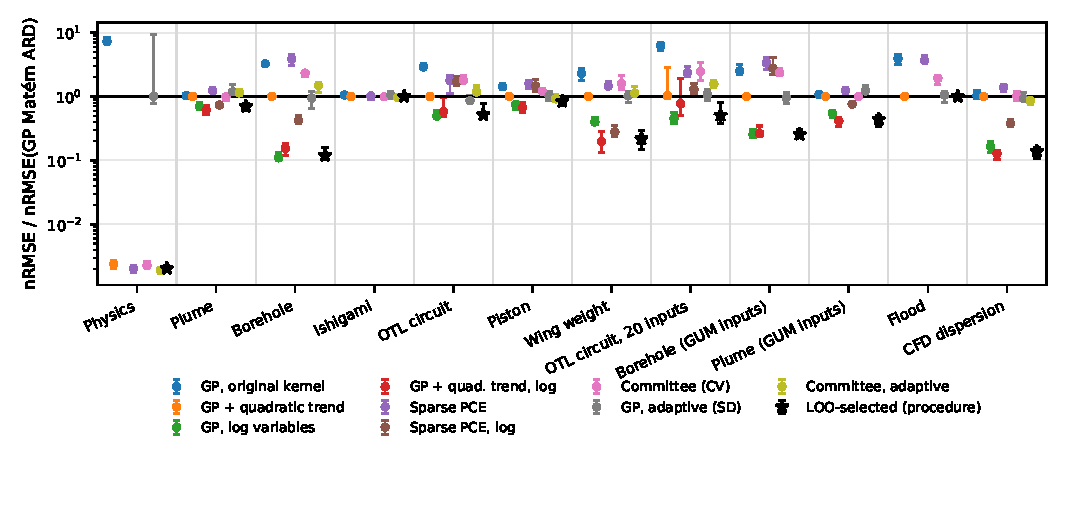
\includegraphics[width=\textwidth]{journal/fig_relative_nrmse}
\caption{nRMSE of each strategy relative to the Mat\'ern ARD GP on the same
design, $N=20$: median over 30 seeds of the paired ratio with 95\%
bootstrap interval. Star: the candidate chosen per seed by the smallest
LOO error (the procedure of Fig.~\ref{fig:flowchart}).}
\label{fig:relative}
\end{figure}

\begin{table}[tb]
\centering
\caption{Validation error of the reported quantities, median over 30 seeds,
$N=20$: relative error (\%) of the mean, SD and $y_{0.95}$ and absolute
error ($\times100$) of $P(Y>T)$ for the recommended GP (log scale for
positive outputs), the same with an AK-MCS design, and the CV-weighted
committee. Generated from the result records.}
\label{tab:prop}
\small
\begin{tabular}{l rrrr r rr}
\toprule
& \multicolumn{4}{c}{GP (passive)} & AK-MCS & \multicolumn{2}{c}{Committee}\\
\cmidrule(lr){2-5}\cmidrule(lr){6-6}\cmidrule(lr){7-8}
Model & mean & SD & $y_{0.95}$ & $P$ & $P$ & $y_{0.95}$ & $P$\\
\midrule
\tabinput{../results/journal/tab_prop.tex}
\bottomrule
\end{tabular}
\end{table}

% journal_results_coverage.tex — results subsection on the validity of the
% surrogate contribution. Numbers: results/journal/summary.json
% ("coverage", "coverage_ranges"); see paper/NUMBERS_journal.md.

\subsection{Is the surrogate contribution valid?}
\label{sec:res-coverage}
Fig.~\ref{fig:coverage} and Table~\ref{tab:coverage} test the three models of
the surrogate error of Section~\ref{sec:contrib} against the true models, for
every surrogate fitted to 20 runs (68 combinations of model and surrogate on
the eleven analytical models, 30 seeds each).

\emph{Pointwise intervals.} The jackknife+ interval covered between 95.2\%
and 99.6\% of the test points (median 97.4\%) in every combination, in line
with its distribution-free guarantee of at least 90\%. The CV-normal interval
covered 89.7--97.1\% (median 94.2\%). The GP's own predictive interval
covered 68--98\% (median 88\%) and fell below 80\% on the plume (both
input models), Ishigami, piston, wing weight and 20-input OTL models: its
posterior SD reflects the fitted covariance, not the actual error. Validity
has a price in width: jackknife+ intervals were a median 1.6 (1.1--2.9)
times as wide as CV-normal ones, and the narrow GP intervals still had the
best interval score~\cite{gneiting2007} in 31 of the 49 GP combinations. For a measurement
uncertainty statement, which claims a coverage probability, the coverage is
the property that matters.

\emph{GUM S1 coverage interval.} Treating the surrogate as exact gave
coverage intervals for $Y$ whose achieved coverage under the reference
distribution ranged from 57\% to 96\% (median 94\%), and standard
uncertainties $u(y)$ that were a median 0.95 times the reference (down to
0.41). Adding the LOO error to every Monte Carlo trial,
equation~\eqref{eq:contrib}, raised the achieved coverage to 91.5--97.3\%
(median 94.9\%) as a normal error and to 91.0--97.0\% (median 94.9\%) by
resampling the residuals, with $u(y)$ a median 1.00 (0.78--1.29) times the
reference. The GP's predictive SD gave 89.8--96.0\% (median 94.6\%). The
largest correction occurred where it is needed most: for the GP with the
original kernel on the Ishigami model, coverage rose from 57\% to 95\%.
Adding the error did not systematically improve exceedance probabilities,
which depend on the tail of the surrogate rather than on its overall
spread.

\emph{Reported quantities.} The difference between the approaches is
largest for the quantities a GUM~S1 evaluation reports. Intervals for
$y_{0.95}$ from joint GP posterior sample paths contained the true value in
a median 63\% of seeds (7--100\%), and those for $P(Y>T)$ in 63\%: the GP
posterior describes the uncertainty of the interpolant as the fitted
covariance model sees it, and is overconfident wherever that model is
misspecified. The jackknife intervals contained the true value in a median
97\% of seeds for both quantities, with the lowest values for the
original-kernel GP, whose error is a bias that no resampling of its own
fits can reveal.

\begin{figure*}[tb]
\centering
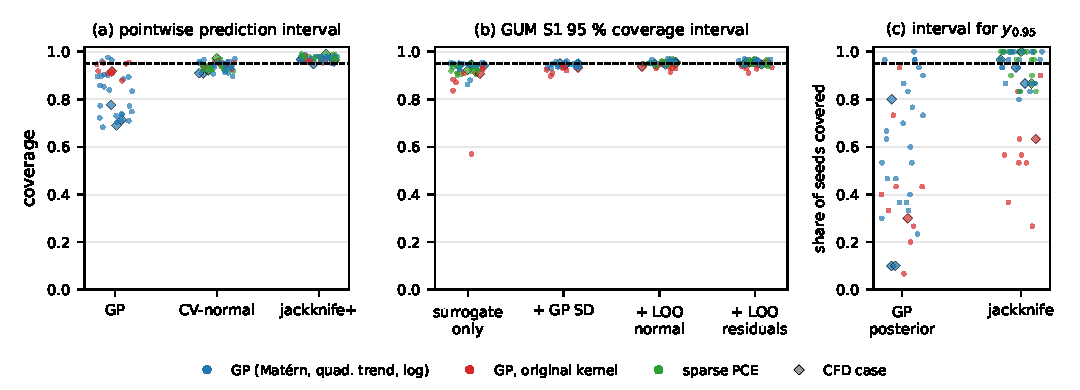
\includegraphics[width=\textwidth]{journal/fig_coverage}
\caption{Coverage of nominal 95\% intervals, mean over 30 seeds; one marker
per combination of model and surrogate (circles: the eleven analytical
models; diamonds: the CFD case, Section~\ref{sec:res-cfd}).
(a) Pointwise prediction intervals on 5000 test points. (b) Achieved
coverage of the GUM~S1 95\% coverage interval of $Y$ under the reference
distribution, with the surrogate treated as exact or with its error added
to each trial. (c) Share of seeds whose 95\% interval for $y_{0.95}$
contains the true value. Dashed line: 0.95.}
\label{fig:coverage}
\end{figure*}

\begin{table*}[tb]
\centering
\caption{Coverage (\%) of nominal 95\% intervals for the GP recommended for
each model (log variables for positive outputs), 30 seeds, $N=20$.
Pointwise: share of test points. GUM~S1: achieved coverage of the 95\%
coverage interval of $Y$. $y_{0.95}$, $P(Y>T)$: share of seeds whose
interval contains the true value (GP: joint posterior paths; J: jackknife).
Generated from the result records.}
\label{tab:coverage}
\scriptsize
\setlength{\tabcolsep}{3.5pt}
\begin{tabular}{l rrr rrrr rr rr}
\toprule
& \multicolumn{3}{c}{Pointwise} & \multicolumn{4}{c}{GUM S1 interval of $Y$} &
\multicolumn{2}{c}{$y_{0.95}$} & \multicolumn{2}{c}{$P(Y>T)$}\\
\cmidrule(lr){2-4}\cmidrule(lr){5-8}\cmidrule(lr){9-10}\cmidrule(lr){11-12}
Model & GP & CV & J+ & exact & +LOO N & +LOO res. & +GP & GP & J & GP & J\\
\midrule
\tabinput{../results/journal/tab_coverage.tex}
\bottomrule
\end{tabular}
\end{table*}

\subsection{Robustness of the surrogate contribution}
\label{sec:res-robust}
\emph{Hyperparameter uncertainty.} Integrating out the GP's hyperparameters
narrowed the gap but did not close it (Table~\ref{tab:bayesgp}). Over the 42
combinations of model and GP candidate at $N=20$, the median pointwise
coverage rose from 80\% with the plug-in hyperparameters to 83\% for the
Student-t process and 96\% for the fully Bayesian GP; the recalibrated GP
reached 95\% (91--98\%) and the jackknife+ 97\%. For the reported quantities
the gain was smaller. Intervals for $y_{0.95}$ contained the true value in
at least 26 of the 30 seeds, the threshold fixed in advance, in 13 of the 42
combinations with the plug-in GP, 15 with the Student-t process, 24 with
the fully Bayesian GP, 23 with the recalibrated GP and 39 with the
jackknife. The fully Bayesian GP fell as low as 8 of 30 seeds (Mat\'ern GP
on the CFD case): averaging over hyperparameters cannot repair a covariance
model that does not fit the response, here the raw scale of a positive,
skewed output. The jackknife fell short of the threshold on three
combinations, all raw-scale GPs on the plume model with GUM-type inputs
and on the Ishigami model (24--25 of 30). By the rule fixed in advance,
none of the GP-based descriptions is a valid surrogate contribution on all
models, and the recommendation of the LOO residuals stands. The coverage
interval of $Y$ itself was robust to the choice: 93\% or more with every
error model. The MCMC chains had integrated autocorrelation times of 38--62
steps, so the 500 steps kept per walker span 8--13 autocorrelation times.

\emph{Number of runs.} The procedure (the candidate with the smallest LOO
error in each seed, with its LOO residuals added) gave GUM~S1 coverage
intervals that covered 93.4--96.9\% of the reference distribution at
$N=10$, 94.2--96.1\% at 20, 94.7--95.7\% at 40 and 94.7--95.1\% at 80, on
every model (Table~\ref{tab:budgets}). Treating the chosen surrogate as
exact covered as little as 81.9\% at $N=10$, against 89.9\% at 20: the
contribution matters most when the budget is smallest. With ten runs, a
design's coverage fell below 90\% in up to 23\% of the designs of a model,
with 20 runs in at most 3\% and with 40 or 80 runs in none. The selection
was within 4.4\% of the best candidate in hindsight at every budget from 20
runs, but up to 37\% worse at $N=10$, where ten LOO residuals rank the
candidates less reliably. A 95\% jackknife+ interval needs at least 19 runs;
with ten it is unbounded. The jackknife intervals for $y_{0.95}$ contained
the true value in 19--30 of 30 seeds at $N=10$ and 23--30 at $N=40$. At
$N=80$ they did so in 14 of 30 seeds on the physics model, whose surrogate
error at that budget (a relative error of $y_{0.95}$ below $10^{-4}$) is at
the level of the observation noise shared by all LOO fits, which no
resampling of the fits can reveal.

\emph{Single designs.} A practitioner has one design. At $N=20$, with the
LOO residuals added, the achieved coverage of the GUM~S1 interval was below
90\% in at most 10\% of the designs of any model and surrogate (median 0\%),
and never below 80.8\%.

\emph{A feature the runs miss.} On the bump model, 13 of the 30 designs of
20 runs placed a run inside the bump. When the design missed it, the GUM~S1
interval still covered 94--95\% of the reference distribution, because the
bump holds only 3\% of the probability mass, and the jackknife+ intervals
95--97\% of the test points; but the intervals for $y_{0.95}$ contained the
true value in only 9--10 of the 17 designs, against 13 of 13 when the bump
was hit. With 40 runs, 6 designs missed the bump, and their intervals for
$y_{0.95}$ contained the true value in 1--4 of 6. Nothing computed from the
runs can flag this: the LOO residuals, like every estimate from the runs,
describe only the errors that the runs reveal. A local feature smaller than
the spacing of the design needs prior knowledge of where to look, or runs
placed there.

\begin{table*}[tb]
\centering
\caption{GP-based descriptions of the surrogate error against the
jackknife, $N=20$, for the GP with a quadratic trend on the recommended
scale (log for positive outputs). Pointwise: mean coverage (\%) of 95\%
prediction intervals on the test points. $y_{0.95}$: seeds (of 30) whose
95\% interval for the 95th percentile contains the true value. Plug-in: ML
hyperparameters; t: Student-t process; MCMC: all hyperparameters
integrated out; recal.: GP SD recalibrated by the LOO standardised
residuals; J+/J: jackknife+ and jackknife. Generated from the result
records.}
\label{tab:bayesgp}
\scriptsize
\setlength{\tabcolsep}{3.2pt}
\begin{tabular}{l rrrrr rrrrr}
\toprule
& \multicolumn{5}{c}{Pointwise coverage (\%)} & \multicolumn{5}{c}{$y_{0.95}$: seeds of 30 covered}\\
\cmidrule(lr){2-6}\cmidrule(lr){7-11}
Model & plug-in & t & MCMC & recal. & J+ & plug-in & t & MCMC & recal. & J\\
\midrule
\tabinput{../results/journal/tab_bayesgp.tex}
\bottomrule
\end{tabular}
\end{table*}

\begin{table}[tb]
\centering
\caption{Achieved coverage (\%) of the GUM~S1 95\% coverage interval of $Y$
for the procedure (candidate chosen by LOO error, LOO residuals added),
mean over 30 seeds, against the number of runs. The CFD case was not run
with 80 runs. Generated from the result records.}
\label{tab:budgets}
\small
\begin{tabular}{l rrrr}
\toprule
Model & $N=10$ & 20 & 40 & 80\\
\midrule
\tabinput{../results/journal/tab_budgets.tex}
\bottomrule
\end{tabular}
\end{table}

% journal_results_cfd.tex — results on the CFD dispersion case (Section 5.6).
% Filled in from results/journal/summary.json once the CFD campaign ends.

\subsection{CFD dispersion case}
\label{sec:res-cfd}
\textit{[Results of the CFD campaign to be inserted.]}

% journal_discussion.tex — Sections 6-8 of the journal manuscript.

\section{Discussion}
\subsection{Relation to the earlier analysis}
\label{sec:earlier}
The earlier analysis made five claims. Three are withdrawn or revised. The
catastrophic GP failure on large domains is a kernel-specification artefact:
with the amplitude estimated, the GP no longer reverts to the mean
(Fig.~\ref{fig:dom}). The spectral acquisition criterion gives no advantage
over plain committee variance on any of the six models on which it was
tested, and is worse on three. The committee's advantage is not general but
comes from a member that matches the dominant term, which a GP with a
quadratic trend or a sparse PCE reproduces on its own. Two claims survive:
aggregation must be error-weighted, and an adaptive committee can be more
accurate than a passive one: it was on four of the seven models on which it
was run, including the CFD case, although it remained less accurate than
the log-variable GP wherever the output is positive, and its exceedance
probabilities were worse on the plume and CFD cases. The records of the earlier
campaigns are kept in the repository~\repocite.

\begin{figure}[tb]
\centering
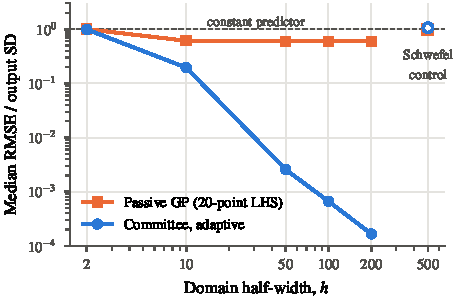
\includegraphics[width=0.62\textwidth]{fig_domain_sweep}
\caption{Physics model on $[-h,h]^3$, $N=20$: median nRMSE over 30 seeds
against the domain half-width, for the GP with the original kernel
(amplitude fixed), the Mat\'ern ARD GP with amplitude, and the committee of
the earlier analysis. Open markers: Schwefel function on $[-500,500]^3$.
Dashed line: constant predictor.}
\label{fig:dom}
\end{figure}

\subsection{What the surrogate contribution should be}
The coverage results separate two uses of a surrogate's uncertainty.
Pointwise, the GP posterior is a useful but uncalibrated description: it
locates where the surrogate is uncertain, which is why it drives good
adaptive designs at larger budgets, but its scale is set by a covariance
model fitted to 20 runs and is too small wherever that model is wrong. For
an uncertainty statement the scale is what matters, and the leave-one-out
residuals estimate it directly, without trusting the covariance model; the
jackknife+ turns them into intervals with a guarantee. The difference is
largest for the reported quantities. A GUM~S1 coverage interval of $Y$ is
fairly robust, because surrogate error that varies across the input space
partly averages out in the distribution of $Y$, and adding the LOO error
to each trial restores its nominal coverage. A 95th percentile or an
exceedance probability is not robust: it depends on the surrogate in a
small region. Intervals from the GP posterior contained the true value in
a median 63\% of the seeds (median over model and surrogate), whereas the
jackknife over LOO fits did so in a median 97\%. Integrating out the
hyperparameters narrowed this gap but did not close it
(Section~\ref{sec:res-robust}): the shortfall comes from covariance models
that do not fit the response, not only from plug-in estimates, and a
Bayesian treatment inherits the covariance model. Rescaling the GP SD by the
LOO standardised residuals, which keeps the GP's localisation of the error
and takes its scale from the runs, came closer, but the jackknife remained
the more reliable description. We therefore recommend the LOO error as the
surrogate contribution, and the jackknife over LOO fits for the uncertainty
of quantities derived from the propagated distribution.

\subsection{Limitations}
The study covers twelve models with up to 20 inputs and budgets of 10 to
80 runs; problems with many more inputs, where sparse and additive
structures matter more, may rank the surrogates differently. Two models were run with
a single budget per input distribution, and the adaptive committees were
run only up to $N=40$ because of their cost. The CFD case is
two-dimensional and steady, with a standard $k$--$\varepsilon$ model; it is a
benchmark with the features a dispersion simulation has, not a validated
prediction for a site, and its reference distribution is built from 800
runs rather than $2\times10^5$. The coverage results are averages over
seeds; for single designs the GUM~S1 interval fell below 90\% in at most
10\% of the designs of a model at $N=20$, and the jackknife+ guarantee (at
least 90\% for nominal 95\%) holds on average over designs, not for every
design. The LOO residuals describe only the errors that the runs can
reveal: a local feature that no run hits goes unnoticed
(Section~\ref{sec:res-robust}), and an error at the level of the
observation noise, shared by all LOO fits, is not seen by the jackknife.
The hyperparameter search ranges were fixed in advance; on the physics
model the amplitude reached the upper end of its range, which understates
the GP there (Section~\ref{sec:res-main}). Several output quantities were
studied on one model only; there, resampling the LOO residual vectors run
by run, which preserves their correlation, gave the nominal coverage of the
GUM~S2 region~\cite{jcgm102}, and resampling the components independently
over-stated the region. The log transformation applies only to positive
outputs, and its back-transformation to the predictive median slightly
underestimates the mean of a skewed output; the bias is included in the
validation errors reported. Finally, the paired tests are exploratory: all
$p$-values were Holm-adjusted together, and nominal differences that do not
survive the adjustment are not claimed.

\section{A procedure for surrogate-based GUM~S1 evaluations}
\label{sec:procedure}
Fig.~\ref{fig:flowchart} condenses the results into a procedure that needs
only the $N$ runs. Its two key steps were validated on the twelve models: the
selection of the surrogate by its LOO error recovered practically all the
benefit of the best specification (Section~\ref{sec:res-select}), and the
LOO error as surrogate contribution restored the nominal coverage of the
GUM~S1 coverage interval (Section~\ref{sec:res-coverage}). Candidates should
include a GP with an estimated amplitude, one length scale per input and a
quadratic trend, and a sparse PCE, each on the log scale when the output
is positive; a fitted hyperparameter at the end of its search range is a
sign that the range should be widened. With fewer than 19 runs a 95\%
jackknife+ interval is unbounded, but the GUM~S1 coverage interval with the
LOO residuals remained valid down to ten runs. The LOO error covers what the
runs can reveal: where a narrow feature is plausible (a narrow plume, a
local flow structure), prior knowledge or runs placed there are needed.
Adaptive designs are optional: a targeted design such as
AK-MCS is worthwhile when a threshold decision is the purpose and the
threshold lies in a tail of the distribution, and
variance-driven designs when the budget is several times the number of
inputs and the model is smooth.

\begin{figure}[tb]
\centering
% fig_flowchart.tex — decision procedure for surrogate-based GUM S1
% propagation (Section "Practical procedure"). \input inside a figure;
% needs \usetikzlibrary{positioning,arrows.meta,shapes.geometric}.
\begin{tikzpicture}[
  node distance=3.2mm and 6mm,
  box/.style={draw, rounded corners=1.5pt, align=center, font=\footnotesize,
              text width=#1, inner sep=2.5pt, fill=white},
  box/.default=54mm,
  dec/.style={draw, diamond, aspect=2.6, align=center, font=\footnotesize,
              inner sep=0.5pt, fill=gray!8},
  side/.style={draw, dashed, rounded corners=1.5pt, align=left, font=\scriptsize,
               text width=30mm, inner sep=2pt},
  arr/.style={-{Latex[length=1.6mm]}, semithick},
  lab/.style={font=\scriptsize}]
\node[box] (start) {Model $Y=f(\mathbf X)$ too costly for $10^5$ Monte Carlo
  trials; budget of $N$ runs};
\node[box, below=of start] (design) {Run $f$ on an $N$-point Latin hypercube
  drawn in the input distribution (inverse-CDF map)};
\node[dec, below=of design] (pos) {$Y>0$, multiplicative?};
\node[box, below=of pos] (fit) {Fit candidates on the log scale if \emph{yes}:
  GP (Mat\'ern-5/2, ARD, estimated amplitude, nugget; $\pm$ quadratic
  trend) and sparse PCE (LAR, corrected LOO); no hyperparameter at the
  end of its search range};
\node[box, below=of fit] (sel) {Keep the candidate with the smallest
  leave-one-out (LOO) error};
\node[dec, below=of sel] (ok) {LOO error fit\\for purpose?};
\node[box, below=of ok] (prop) {GUM S1 propagation through the surrogate,
  adding to every trial a draw of the LOO residuals};
\node[box, below=of prop] (rep) {Report $y$, $u(y)$ and the coverage
  interval (trials by GUM S1 7.9); state the surrogate contribution;
  intervals for derived quantities by the jackknife over the LOO fits};
\node[side, right=of ok] (more) {Add runs, e.g.\ while the surrogate
  share of $u^2(y)$ exceeds 1\%: extend the design (space filling); a
  targeted design only for a threshold decision};
\node[side, right=of prop] (no) {Not the GP posterior SD, nor a committee
  envelope: both understate the surrogate error};
\draw[arr] (start) -- (design);
\draw[arr] (design) -- (pos);
\draw[arr] (pos) -- (fit);
\draw[arr] (fit) -- (sel);
\draw[arr] (sel) -- (ok);
\draw[arr] (ok) -- node[lab, right] {yes} (prop);
\draw[arr] (prop) -- (rep);
\draw[arr] (ok) -- node[lab, above] {no} (more);
\draw[arr] (more.north) |- (design.east);
\draw[dashed] (no.west) -- (prop.east);
\end{tikzpicture}

\caption{Procedure for a GUM~S1 evaluation with a surrogate fitted to $N$
runs of an expensive model.}
\label{fig:flowchart}
\end{figure}

\subsection{Worked example}
\label{sec:worked}
The procedure is implemented in \texttt{src/procedure.py} of the
repository~\repocite; given the $N$ runs and a sampler of the input
distribution, it returns the GUM~S1 results with and without the surrogate
contribution, jackknife intervals of the reported quantities and an
uncertainty budget. The number of Monte Carlo trials is chosen by the
adaptive procedure of GUM~S1~\cite{jcgm101} (clause 7.9) for a stated number
of significant digits of $u(y)$. Applied to the CFD case with the 20 runs
of the first design, it chose the log-scale GP with a quadratic trend, whose LOO RMSE (23\,mg\,m$^{-3}$) was smaller than those of the
log-scale GP (31), the log-scale sparse PCE (93) and the raw-scale
candidates (157--260). Two significant digits of $u(y)$ (numerical
tolerance 5\,mg\,m$^{-3}$) took 115 batches of $10^4$ trials, $M=1.15\times10^6$;
the upper limit of the coverage interval was the last quantity to settle.
Table~\ref{tab:worked} compares the result with the reference, which a
practitioner would not have. Adding the LOO residuals changed the reported
quantities by at most 1.3\%; here it lowered them,
because the residuals have a negative mean ($-0.013$ on the log scale,
mostly from one run). The reported 95\% coverage interval contains
94.3\% of the reference distribution. The jackknife intervals, which
describe the surrogate error alone, contain the reference values of the
mean, the lower limit of the coverage interval and $P(C>\mathrm{IDLH})$;
for the SD, the 95th percentile and the upper limit the reference lies
0.7--1.6\% above the upper end of the interval, by less than half the
standard uncertainty of the reference itself.

The GUM uncertainty framework, the law of propagation of uncertainty applied
to the same surrogate at the input means, gives $y=318$\,mg\,m$^{-3}$,
$u(y)=232$\,mg\,m$^{-3}$ and the interval $y\pm1.96\,u(y)=[-137,772]$\,mg\,m$^{-3}$,
which contains only 85.5\% of the reference distribution and extends to
impossible negative concentrations. For this skewed output the Monte Carlo
method of GUM~S1, and therefore a surrogate, is needed.

The budget treats the surrogate error $E$ as one more input quantity of
the model~\eqref{eq:contrib}, with $E$ drawn from the LOO residuals, and gives first-order variance shares of the inputs and the
total share of $E$ (estimators of Saltelli et al.~\cite{saltelli2010}).
The reference wind speed contributed 36\% of $\mathrm{Var}(Y)$, the release
rate 29\%, the receptor distance 5.9\%, the turbulent Schmidt number 4.2\%,
the building height 3.2\% and the roughness length 1.7\%; interactions
between the inputs 20\% and the surrogate 0.3\%. With this surrogate, then,
the evaluation is limited by the input uncertainties rather than by the
number of runs, and further CFD runs would mainly narrow the jackknife
intervals of the tail quantities. The budget is how a practitioner can
tell whether more runs are worth their cost: a surrogate share comparable
to those of the inputs would indicate the opposite.

\begin{table}[tb]
\centering
\caption{Worked example: the procedure of Fig.~\ref{fig:flowchart} on the
CFD case with $N=20$ runs and $M=1.15\times10^6$ trials, chosen by the
adaptive procedure of GUM~S1 (mg\,m$^{-3}$). Columns:
surrogate treated as exact; with the LOO residuals added (the reported
result); 95\% jackknife interval over the LOO fits (surrogate error only);
reference from 800 CFD runs with its standard uncertainty in parentheses.}
\label{tab:worked}
\small
\begin{tabular}{l rr c r}
\toprule
Quantity & exact & with $E$ & jackknife & reference\\
\midrule
\tabinput{../results/journal/tab_worked.tex}
\bottomrule
\end{tabular}
\end{table}

% journal_conclusion.tex — Section 8.

\section{Conclusion}
\label{sec:conclusion}
\textit{[To be completed with the CFD results.]}

